\documentclass[a4paper]{article}

\usepackage[utf8]{inputenc}

\usepackage{url}
\usepackage[hidelinks]{hyperref}

\usepackage{caption}

\usepackage{listings}

\usepackage{color}

% *** GRAPHICS RELATED PACKAGES ***
%\usepackage[pdftex]{graphicx}
\usepackage{graphicx}
%\usepackage[dvips]{graphicx}
% to place figures on a fixed position
\usepackage{float}

\usepackage[margin=1in]{geometry}

\title{IoT Lab}
\author{}
\date{}


\begin{document}

\maketitle

\tableofcontents

\section{IoT lab measurement exercises}

In the first phase of the lab a micro-controller will be transformed into a mote. A sensor mote is capable of detect various parameters of its environment and is capable of communication. For this purpose a sensor and a radio module is going to be attached to the micro-controller. For this same device an actuator is going to be connected to it. Furthermore a simple display device is also connected to the already built hierarchy.

In the second phase of the lab a virtual device is created using one of the cloud IoT provider's services that is going to accept and process the data arriving from our physical sensor. The service is going to store and display the data. Furthermore a virtual controller is attached to the virtual sensor that is going to send control signals for the physical device. A gateway device is used for translating the data into the right format between the physical and virtual devices.

The arrangement of these components can be seen on Figure~\ref{fig:meas-arrangement}. The task of the students attending this lab is to program the devices and the gateway for the achieving the desired operation.

\begin{figure}[H]
    \centering
    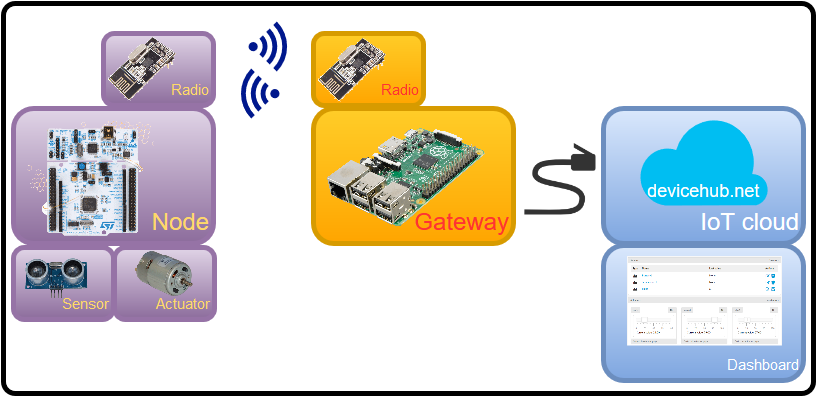
\includegraphics[width=0.9\textwidth]{figures/devices-arrangement.png}
    \caption{Arrangement of devices and components used in this lab}
    \label{fig:meas-arrangement}
\end{figure}

\section{Further Reading}

\begin{itemize}
    \item \href{https://qosip.tmit.bme.hu/foswiki/pub/Meres/OpenFlowMScMeresiSegedlet/a19-lantz.pdf}{A Network in a
              Laptop: Rapid Prototyping for Software-Defined Networks}
    \item

          \href{https://qosip.tmit.bme.hu/foswiki/pub/Meres/OpenFlowMScMeresiSegedlet/mininet-hotnets2010-final.pdf}{Presentation
              of conference proceedings on Mininet}
    \item	Mininet page: \url{http://mininet.org/}
    \item	Mininet wiki: \url{https://github.com/mininet/mininet/wiki}
    \item	Mininet introduction: \url{https://github.com/mininet/mininet/wiki/  Introduction-to-Mininet}
    \item	Mininet Python API: \url{http://mininet.org/api/hierarchy.html}
\end{itemize}

OpenFlow specifications:
\begin{itemize}
    \item
          \href{https://qosip.tmit.bme.hu/foswiki/pub/Meres/OpenFlowMScMeresiSegedlet/openflow-spec-v1.0.0.pdf}{v1.0}
    \item
          \href{https://qosip.tmit.bme.hu/foswiki/pub/Meres/OpenFlowMScMeresiSegedlet/openflow-spec-v1.1.0.pdf}{v1.1}
    \item

          \href{https://qosip.tmit.bme.hu/foswiki/pub/Meres/OpenFlowMScMeresiSegedlet/openflow-switch-v1.3.4.pdf}{v1.3.4}
    \item

          \href{https://qosip.tmit.bme.hu/foswiki/pub/Meres/OpenFlowMScMeresiSegedlet/openflow-switch-v1.4.1.pdf}{v1.4.1}
    \item

          \href{https://qosip.tmit.bme.hu/foswiki/pub/Meres/OpenFlowMScMeresiSegedlet/openflow-switch-v1.5.1.pdf}{v1.5.1}

\end{itemize}

\appendix

\section{Entry quiz sample questions}

\begin{enumerate}
    \item Describe briefly the main concept of the OpenFlow recommendation.
    \item What are the components of an OpenFlow network?
\end{enumerate}

\section{Lab exercises}

\subsection{Lab environment}

\end{document}